% Created 2013-12-20 金 04:52
\documentclass[12pt]{jsarticle}
\usepackage[dvipdfmx]{graphicx}
\usepackage{comment}
%\usepackage{setspace}
%%\date{\today}
%\title{}
\textheight = 25truecm
\textwidth = 18truecm
\topmargin = -1.5truecm
\oddsidemargin = -1truecm
\evensidemargin = -1truecm
\marginparwidth = -1truecm
\def\theenumii{\Alph{enumii}}
\def\theenumiii{\alph{enumiii}}
\def\labelenumi{(\theenumi)}
\def\labelenumiii{(\theenumiii)}
%\setstretch{0.9}
\setlength\intextsep{0pt}
\setlength\textfloatsep{0pt}

\newcommand{\insertfigurecontents}[5][1]{
  \includegraphics[clip,width=#1\columnwidth]{\figdir/#3.\figext}
  \caption{#4}\ecaption{#5}\label{#2}
}

\newcommand{\insertfigure}[5][0.9]{
  \begin{figure}[tb]
    \begin{center}
      \insertfigurecontents[#1]{#2}{#3}{#4}{#5}
    \end{center}
  \end{figure}
}

\newcommand{\insertwidefigure}[5][0.9]{
  \begin{figure*}[tb]
    \begin{center}
      \insertfigurecontents[#1]{#2}{#3}{#4}{#5}
    \end{center}
  \end{figure*}
}
\begin{document}

%\maketitle
%\tableofcontents

\begin{center}
%%%%%%%%%%%%%%%%%%%%%%%%%%%%%%%%%%%%%%%
%%%タイトル                         %%%
%%%%%%%%%%%%%%%%%%%%%%%%%%%%%%%%%%%%%%%
{\LARGE 2015年度前期研究計画(藤田)}
\end{center}

\begin{flushright}
  2015/4/6\\
  藤田将輝
\end{flushright}
%%%%%%%%%%%%%%%%%%1章%%%%%%%%%%%%%%%%%%%
\section{はじめに}
本資料では,博士前期課程における藤田の研究計画を示す.
2015年度前期は,デバッグ支援環境における,パケットの
受信処理の実装を行う.
また,本環境におけるパケット受信割り込み処理にかかる時間と,
実際のNICを用いたパケット受信処理にかかる時間とを比較し,評価する.
この評価からSWoPP2015の原稿を執筆する.
その後は,本環境を用いて,NICの受信割り込み処理におけるバグを再現する.
また,割り込みレベルに起因するバグの再現を可能にしようと考えているが,
調査が未完了であるため,詳細な計画を立てることができない.
このため,調査が完了した後,再度研究計画を立てる.

\section{課題一覧}
藤田の課題一覧を別紙の表「課題一覧(藤田)(2015年4月6日)」に示し,
課題について以下で説明する.
\begin{description}
    \item[(大課題1)]Mintを用いたデバッグ手法の提案\\
        OSのデバッグを行う際に,特に困難であるのが,割り込み処理に関する
        デバッグである.割り込み処理は非同期な処理であり,いつ発生するかが
        予想できない.そこで,Mintを用いて,デバッグ支援OSとデバッグ対象OS
        を動作させ,任意のタイミングで割り込み処理を発生させる環境を
        構築し,デバッグを支援する.今回のデバッグ対象はNICドライバの
        パケット受信割り込み処理としている.
        現在は,受信割り込み処理の発生までを完了しているが,
        パケットの受信が未完了である.
        これを完了させた後,割り込みを発生させてから,割り込み処理が
        完了するまでにかかる時間を測定し,
        実際のNICを用いたパケット受信割り込み処理にかかる時間と比較し,
        評価する.
\end{description}
\section{今後の予定}
今後の予定について,図\ref{fig:plan}に示し,以下で説明する.
%\insertwidefigure[0.75]{plan}{fig/fig1}{2015年度前期研究計画}{Plan\_of\_research\_2015}
\begin{figure}[t]
    \begin{center}
    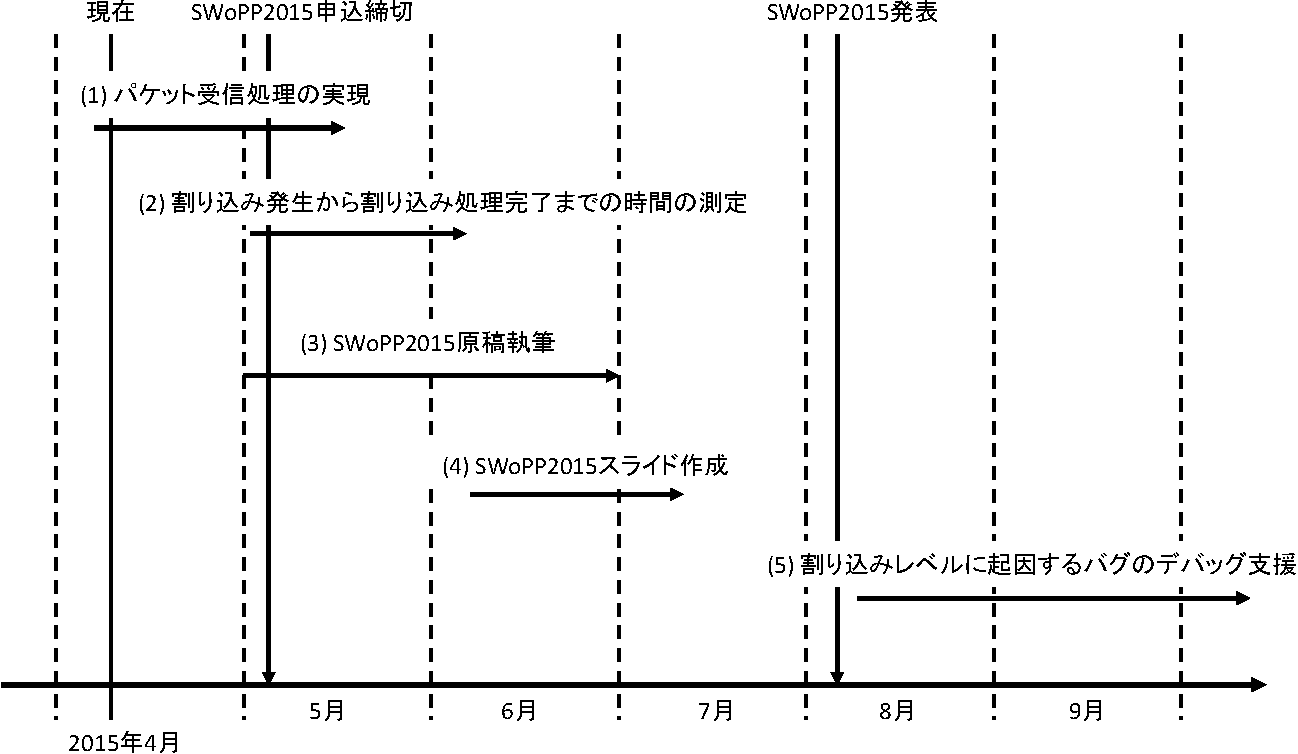
\includegraphics[clip,scale=0.65]{fig/fig1.pdf}
    \caption{2015年度前期研究計画}
    \label{fig:plan}
\end{center}
\end{figure}
\begin{enumerate}
    \item パケット受信処理の実現(2015年5月中旬)\\
        Etherフレームの構造を擬似したものを作成し,処理させる.
        パケットの種類はUDPとする.
    \item 本環境における,割り込み発生から割り込み処理完了までの時間の測定\\
        本環境を用いて,パケットを共有メモリに配置し,IPIを送信し,
        NICドライバに受信処理をさせる.
        この際にかかる時間を測定する.
        また,測定した時間と,実際のNICを用いたパケット受信割り込み処理に
        かかる時間とを比較し,評価する.
    \item SWoPP2015原稿執筆(2015年6月下旬)
    \item SWoPP2015の発表スライド作成(2015年7月上旬)
    \item 割り込みレベルに起因するバグのデバッグ支援(未定)\\
        割り込みレベルに起因するバグについて調査し,Mintを用いて,
        調査したバグを再現する.
\end{enumerate}
\section{おわりに}
本資料では,博士前期課程における藤田の研究計画を示した.
\end{document}


